\apendice{Especificación de diseño}

\section{Introducción}

\section{Diseño de datos}

Para el desarrollo de la aplicación Android no podemos hablar estrictamente de un diseño de los datos, ya que se trata de un cliente que no interactúa directamente con la base de datos, sino que lo hace a través de la API del servidor, la cual devuelve siempre todos los datos en un objeto con formato JSON. En este sentido, podemos abstraernos del diseño e implementación concretas de la base de datos, ya que nuestra gestión de los datos solo depende de las características del JSON que nos va a devolver cada petición. La estructura de la respuesta de cada petición a la API se especifica en el Manual del programador de mi compañero José Luis Garrido Labrador. 

\section{Diseño procedimental}

Tal y como se ha planteado la aplicación de Android, existen dos procesos relevantes que es importante entender, ya que supondrán la base del funcionamiento de la aplicación. 

\begin{itemize}
	\item En primer lugar, la llamada a los servicios genéricos de la API. Todas las interacciones con la lógica de negocio de la aplicación (iniciar sesión, visualizar usuarios, añadir usuarios...) se realizan de esta manera. Por esta razón, para garantizar el buen funcionamiento de la aplicación, este proceso debe incluir una comprobación sobre si existe conexión a internet, si la sesión está activa y si la respuesta de la API es la esperada. Esta interacción se representa en el diagrama de secuencias de la figura~\ref{fig:sequenceAPI}. 
	\item En segundo lugar, la petición y recepción de los datos de una cama en tiempo real. Este proceso se realiza a través de conexión a nivel de \textit{sockets} con el servidor y la gestión de eventos empleando la librería Socket.IO. Esta interacción se representa en el diagrama de secuencias de la figura~\ref{fig:sequenceStreaming}. 
\end{itemize}

\begin{figure}
	\centering
	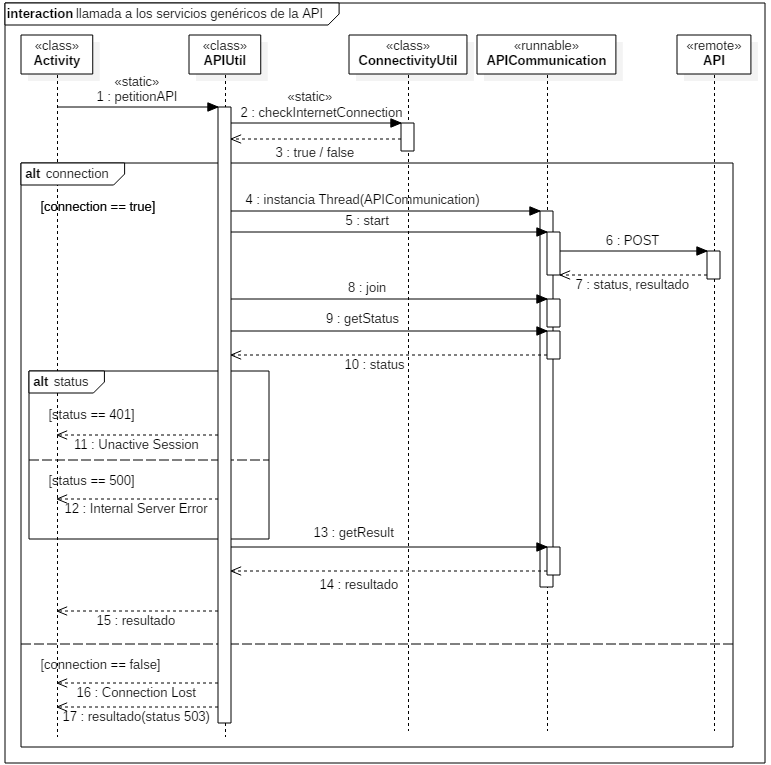
\includegraphics[width=1.3\textwidth]{../img/sequenceAPI.png}
	\caption{Diagrama de secuencias, llamada a los servicios genéricos de la API.}
	\label{fig:sequenceAPI}
\end{figure}

\begin{figure}
	\centering
	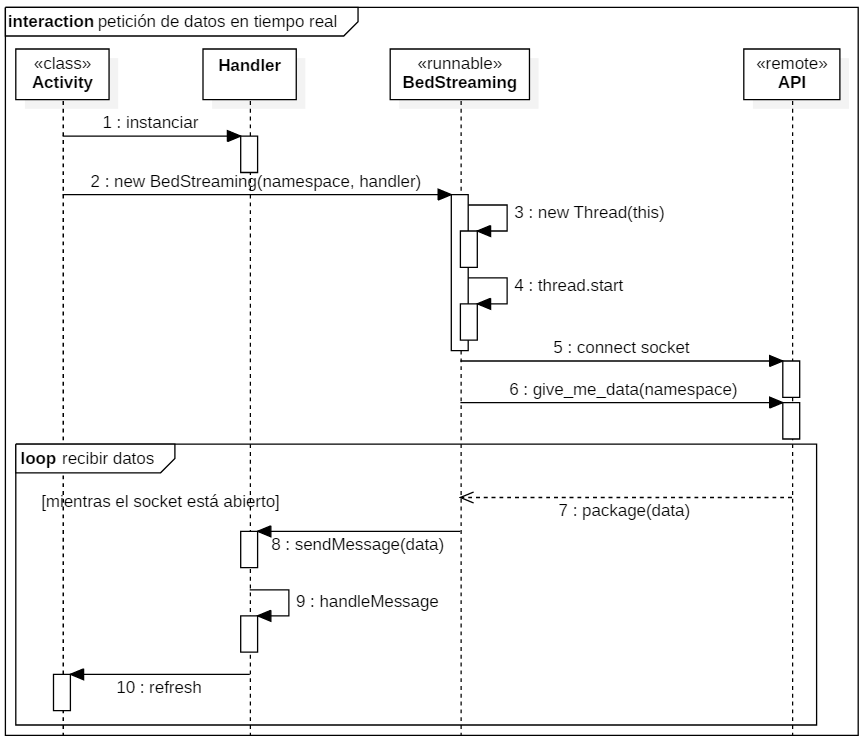
\includegraphics[width=1\textwidth]{../img/sequenceStreaming.png}
	\caption{Diagrama de secuencias, petición de datos en tiempo real.}
	\label{fig:sequenceStreaming}
\end{figure}

El funcionamiento del resto de procesos es fácilmente deducible a partir del código o corresponde con el uso de elementos propios del \textit{framework} de Android. La especificación y funcionamiento de estos elementos se puede consultar en la página web oficial de \textit{Android Developers}~\cite{androiddevelopers}.  

\section{Diseño arquitectónico}

\section{Diseño de interfaces}

Inicialmente se realizaron una serie de prototipos básicos en los que se plasmaron las principales funcionalidades de la aplicación, sin prestar especial atención a los aspectos estéticos de la misma. Para ello se usó la herramienta de prototipado Pencil, ya que permite incorporar elementos propios de la guía de estilos que se ha seguido para el diseño de las interfaces de usuario: \textit{Material Design}. 

\begin{figure}
	\centering
	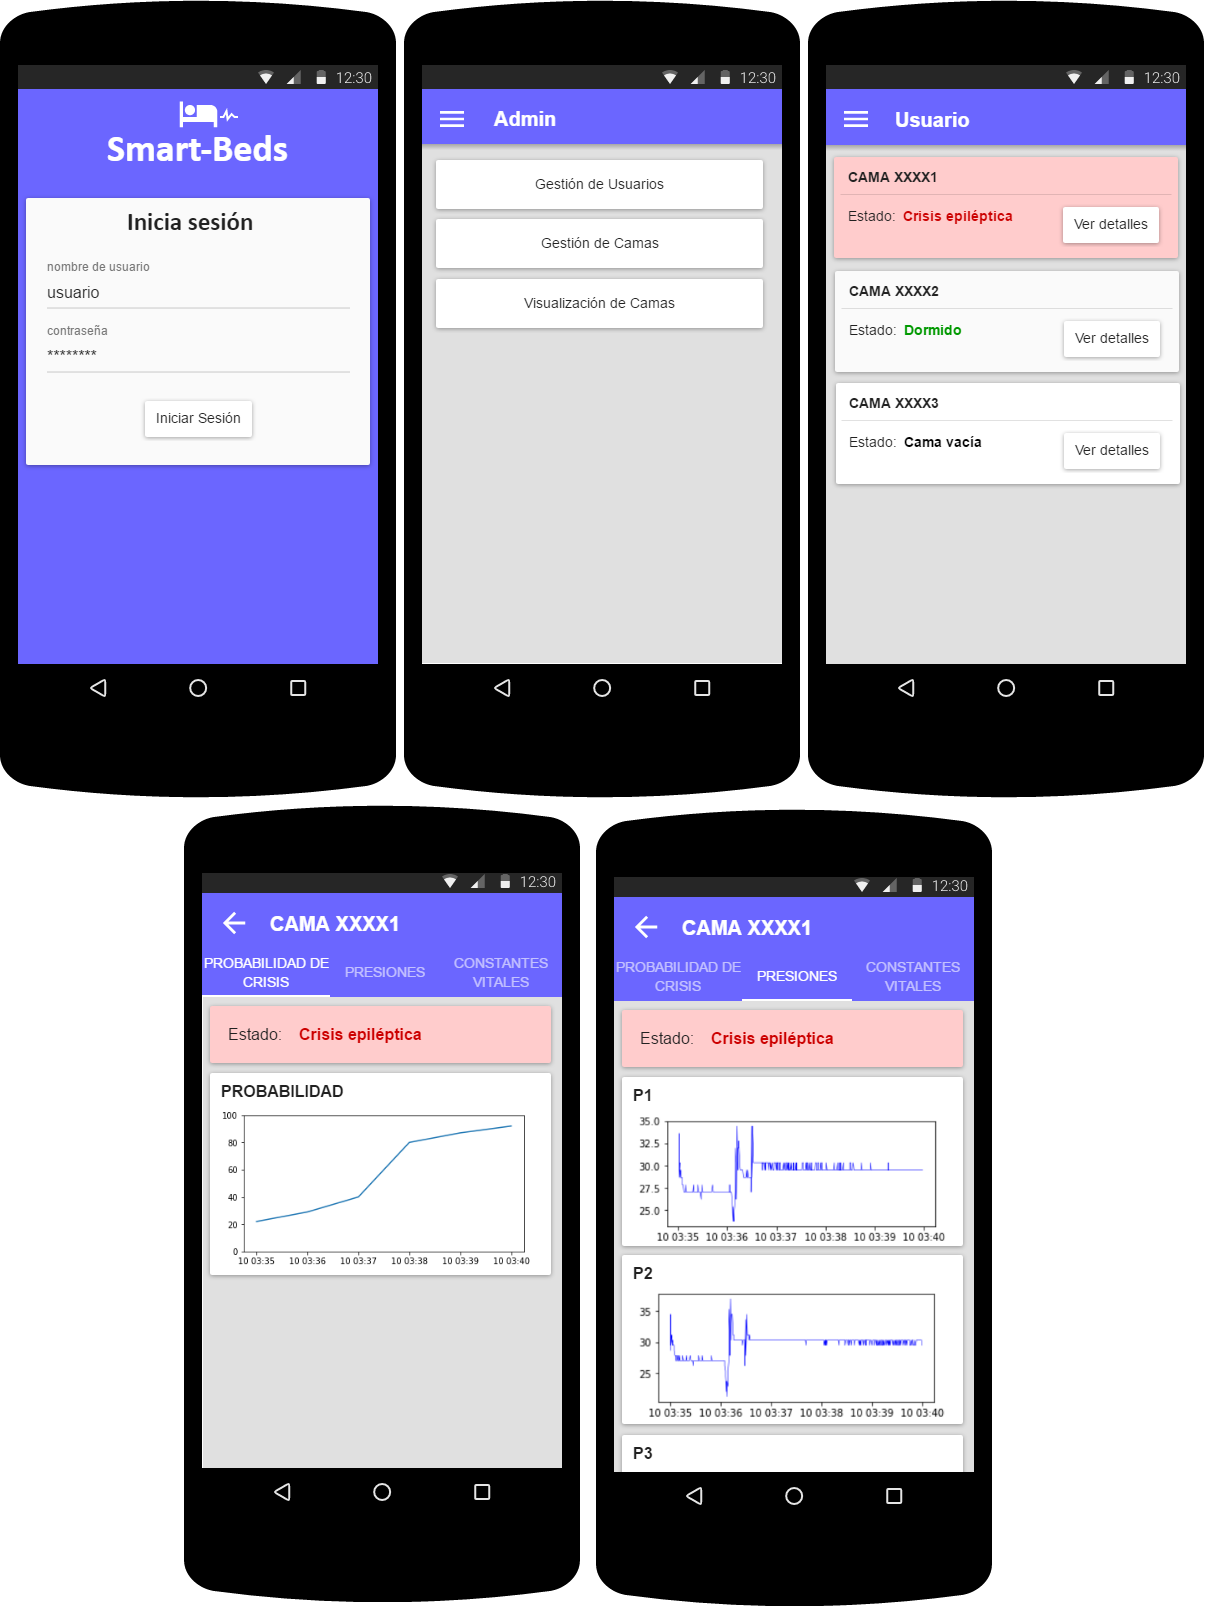
\includegraphics[width=1\textwidth]{../img/prototipos.png}
	\caption{Prototipos iniciales de las pantallas de: login, administración, visualización de camas y visualización de datos.}
	\label{fig:prototipos}
\end{figure}
